\section{Development from a Prior Design}\label{sec:development}

\subsection{Baseline: always-on banding}\label{sec:prior}
\scl{} was developed from an earlier design of the same research program,
called always-on banding (\aob{}). \aob{} computed the same nested Otsu bands
but treated every stream as noisy. In every frame it applied the bands,
removed every weaker candidate that overlapped a stronger one with IoU above
one half, and remapped all scores by rank onto fixed ranges. It admitted no
candidate at the first frame. \aob{} was designed for noisy detector streams,
and it is the baseline of this section.

Table~\ref{tab:prior} compares \aob{} and \scl{} with the same strong published
trackers on MOT17 \cite{milan2016mot16}. \aob{} lowered the HOTA of
SparseTrack by 4.15 points and that of BoostTrack by 5.89 points online and
5.37 points with interpolation, all with intervals below zero. Two causes were
found. First, overlap-based duplicate removal deleted occluded people in
crowds. Second, the self-calibrated thresholds were stricter than the
trackers' own: for SparseTrack and online BoostTrack, false positives fell by
1,630 and 1,351, but false negatives rose by 4,955 and 6,167. On the same
trackers, \scl{} changed HOTA by $+0.06$ for SparseTrack and left both
BoostTrack variants identical to the host. Figure~\ref{fig:prior} shows the
same comparison.

\begin{table}[t]
\caption{Baseline comparison of the development stage on MOT17 val-half
(published YOLOX-X detections). Host: published tracker alone (our
reproduction). $\Delta$: tracker with the prior design \aob{} or with \scl{}
minus host, with 95\% paired-bootstrap interval (10,000 resamples,
seed 42). Bold intervals exclude zero.}
\label{tab:prior}
\centering\footnotesize
\setlength{\tabcolsep}{3pt}
\renewcommand{\arraystretch}{1.1}
\begin{tabular}{@{}lrcc@{}}
\toprule
Metric & Host & $\Delta$ \aob{} & $\Delta$ \scl{}\\
\midrule
\multicolumn{4}{@{}l}{\textit{SparseTrack} \cite{liu2025sparsetrack}}\\
\quad HOTA & 68.88 & \cibt{-4.15}{-5.54}{-1.66} & \cit{+0.06}{-0.01}{+0.25}\\
\quad MOTA & 77.85 & \cibt{-6.14}{-8.10}{-2.74} & \cit{+0.08}{-0.03}{+0.30}\\
\quad IDF1 & 81.97 & \cibt{-4.49}{-6.19}{-1.96} & \cit{+0.16}{-0.02}{+0.70}\\
\multicolumn{4}{@{}l}{\textit{BoostTrack, online} \cite{stanojevic2024boosttrack}}\\
\quad HOTA & 68.49 & \cibt{-5.89}{-7.76}{-2.87} & 0 (identical)\\
\quad MOTA & 75.50 & \cibt{-8.87}{-12.37}{-7.14} & 0 (identical)\\
\quad IDF1 & 81.41 & \cibt{-6.22}{-9.33}{-2.85} & 0 (identical)\\
\multicolumn{4}{@{}l}{\textit{BoostTrack, with interpolation} \cite{stanojevic2024boosttrack}}\\
\quad HOTA & 71.72 & \cibt{-5.37}{-7.30}{-2.75} & 0 (identical)\\
\quad MOTA & 81.03 & \cibt{-8.73}{-12.59}{-6.50} & 0 (identical)\\
\quad IDF1 & 84.16 & \cibt{-5.65}{-8.96}{-2.77} & 0 (identical)\\
\bottomrule
\end{tabular}
\end{table}


\begin{figure}[t]
\centering
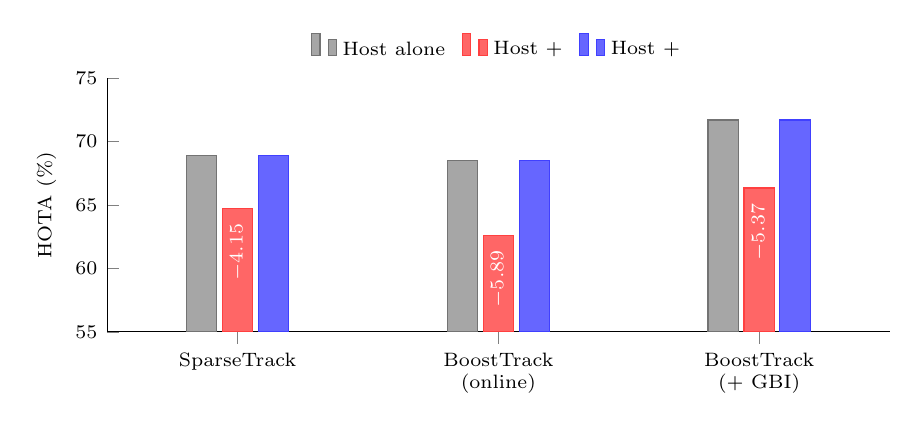
\begin{tikzpicture}
\begin{axis}[
  ybar,
  /pgf/bar width=11pt,
  width=0.95\columnwidth,
  height=4.8cm,
  ymin=55, ymax=75,
  xmin=0.5, xmax=3.5,
  xtick={1,2,3},
  xticklabels={SparseTrack, {BoostTrack\\(online)}, {BoostTrack\\(+ GBI)}},
  xticklabel style={align=center},
  ylabel={HOTA (\%)},
  axis x line*=bottom,
  axis y line*=left,
  tick label style={font=\scriptsize},
  label style={font=\scriptsize},
  legend style={at={(0.5,1.03)}, anchor=south, legend columns=3,
    font=\scriptsize, draw=none, /tikz/every even column/.append style={column sep=4pt}},
  legend cell align=left,
]
\addplot[fill=black!35, draw=black!55] coordinates {(1,68.88) (2,68.49) (3,71.72)};
\addplot[fill=red!60, draw=red!75] coordinates {(1,64.72) (2,62.61) (3,66.35)};
\addplot[fill=blue!60, draw=blue!75] coordinates {(1,68.93) (2,68.49) (3,71.72)};
\legend{Host alone, Host + \aob{}, Host + \scl{}}
\node[rotate=90, anchor=east, font=\scriptsize, text=white] at (axis cs:1,64.3) {$-4.15$};
\node[rotate=90, anchor=east, font=\scriptsize, text=white] at (axis cs:2,62.2) {$-5.89$};
\node[rotate=90, anchor=east, font=\scriptsize, text=white] at (axis cs:3,65.9) {$-5.37$};
\end{axis}
\end{tikzpicture}

\caption{HOTA on MOT17 val-half of three strong published trackers alone, with
\aob{}, and with \scl{}. The labels give the change caused by \aob{}.}
\label{fig:prior}
\end{figure}

\subsection{Design steps}\label{sec:steps}
Each step from \aob{} to \scl{} was introduced to remove one diagnosed cause
and was compared with the step before it on development data
(Table~\ref{tab:ablation}). Emulating \aob{} inside the new framework reduced
ByteTrack at floor 0.1 from 67.70 to 56.41 HOTA and OC-SORT from 66.44 to
45.72. The regime gate, which adds the regime estimate, the self-limiting
clean regime, and the crowd-safe duplicate rule, restored SparseTrack from
64.72 to 68.93 and BoostTrack from 62.61 to 68.37. Estimating the regime from
the whole stream removed regime changes in the middle of a stream and raised
ByteTrack from 67.561 to 67.702 and OC-SORT from 65.697 to 66.071. The
continuation rescue added 0.2 to 0.4 points for OC-SORT. The background check
completed \scl{}: it returned ByteTrack and BoostTrack to output identical to
the host and raised OC-SORT to 67.04 and 66.91 at the two floors. Four
variants were rejected on evidence, because they lowered HOTA, added false
positives, or let false tracks through on a noisy stream.

\begin{table*}[t]
\caption{Design steps from always-on banding (\aob{}) to \scl{} on development
data (HOTA, \%), and variants that were tested and rejected. The floor of
ByteTrack and OC-SORT is given in parentheses.}
\label{tab:ablation}
\centering\footnotesize
\setlength{\tabcolsep}{4pt}
\begin{tabular}{@{}>{\raggedright\arraybackslash}p{30mm}>{\raggedright\arraybackslash}p{44mm}>{\raggedright\arraybackslash}p{78mm}@{}}
\toprule
Step & Change & Effect\\
\midrule
\aob{} emulated & always-noisy bands, overlap deduplication, rank remap & ByteTrack (0.1) 56.41 vs host 67.70; OC-SORT (0.1) 45.72 vs 66.44\\
+ regime gate & regime statistic, host-anchored clean regime, crowd-safe duplicates & SparseTrack 64.72 to 68.93 (host 68.88); BoostTrack 62.61 to 68.37 (host 68.49)\\
+ whole-stream regime & regime from all past frames & ByteTrack (0.1) 67.561 to 67.702; OC-SORT (0.1) 65.697 to 66.071\\
+ continuation rescue & foreground track-consistent rescue & OC-SORT (0.01) 66.405 to 66.619; OC-SORT (0.1) 66.071 to 66.469\\
+ background check = \scl{} & no background mode gives no evidence against the host & ByteTrack/BoostTrack (0.1) identical to host; OC-SORT 67.041 (0.01), 66.907 (0.1)\\
\midrule
\multicolumn{2}{@{}l}{\textit{Rejected variant}} & \textit{Evidence}\\
\multicolumn{2}{@{}l}{no candidates at frame 1} & $-0.3$ to $-0.5$ HOTA on every MOT17 host\\
\multicolumn{2}{@{}l}{rescue below a two-stage host's low stage} & FP $+700$ to $+1000$, $-0.4$ to $-0.5$ HOTA\\
\multicolumn{2}{@{}l}{rank-remapped scores in clean frames} & ByteTrack $-0.2$ / $-1.6$ HOTA\\
\multicolumn{2}{@{}l}{host-clipped noisy primary band} & KITTI YOLOv8n ByteTrack $+1.4$ HOTA but uncontrolled false tracks on a noisy aerial stream (26.9 vs 14.9 boxes/frame)\\
\bottomrule
\end{tabular}
\end{table*}


\subsection{Freeze and tests}\label{sec:freeze}
The final configuration was frozen before any external evaluation. It was
recorded in a version-control tag and protected by a lock file that holds
cryptographic hashes of the layer, its configuration, and the evaluation
runners. Every later run verified the lock before running. Sixty-one automated
tests check that the layer uses no future data, that its state resets between
sequences, that clean streams pass through unchanged, that the output does not
depend on detector, tracker, or sequence names, that affine score transforms
leave the bands unchanged where designed, and that the lock is intact.
